\section{Evaluation}
\label{section:evaluation}
In the following chapter the mobile implication of \gls{see} will be evaluated in a user study.
Therefore, the mobile application will be compared with the desktop version.

This chapter will start with a description of the desktop version and its main differences in section \ref{desktop}.
Continuing with a defined aim and the precise hypotheses for the user study in section \ref{aim}.
After sketching the first experiment set up in section \ref{experiment} the actual experiment set up will be discussed in detail in section \ref{real} including the used survey tool, questionnaires and the pilot study.
\subsection{SEE Desktop}
\label{desktop}
In this section the desktop version of \gls{see} will be explained.
In this evaluation the mobile version of \gls{see} will be compared with the desktop version.
Therefore, it is necessary to take a deeper look at the differences between those two versions.
Especially at how the interactions differ and what impact it could have on the user experience.

One outstanding difference from the desktop version to the mobile version is the selection of the interaction modes.
While in the mobile version the menu for the interaction modes is always visible in the desktop version by pressing space a menu screen opens as seen in figure \ref{fig:menu}.
Alternatively interaction modes can be changed by pressing one of the "1-9" keys, which, however requires the user to memorize which number belongs to which mode.

\begin{figure}[htb]
  \centering
  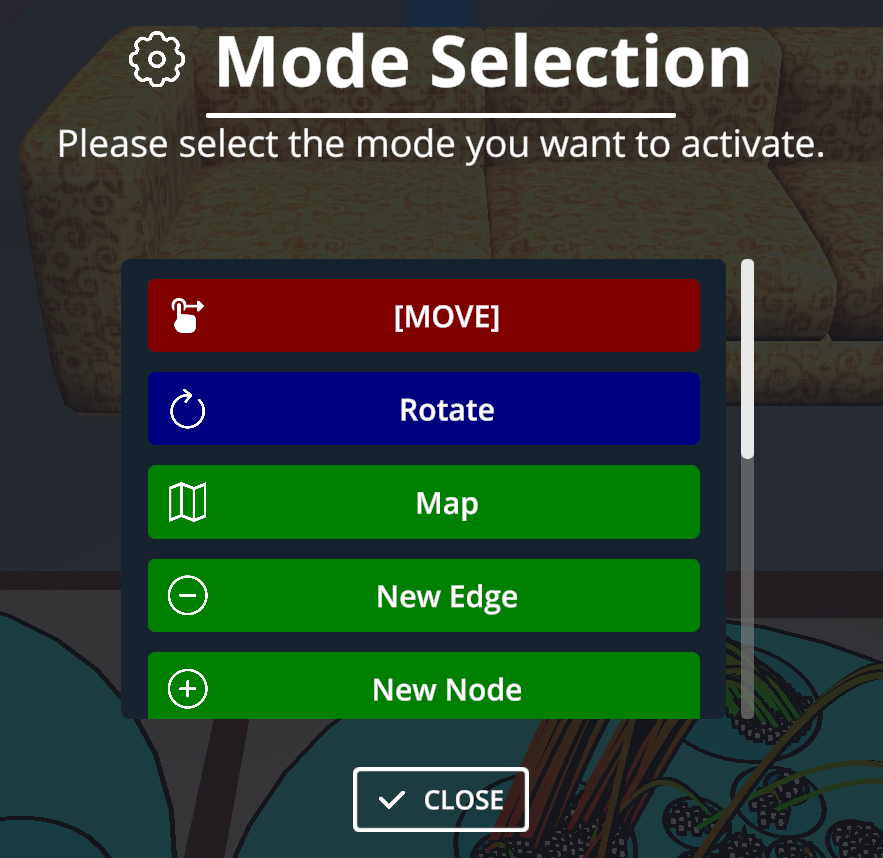
\includegraphics[width=0.8\textwidth]{Evaluation/img/menu.png}
  \caption{The desktop menu for selecting interaction modes.}\label{fig:menu}
\end{figure}

Another difference is the type of user input.
The desktop version uses mouse hovering to display the name of a hovered \gls{node} or \gls{plane}.
This is a faster method then touching the object first in the mobile version.
In addition to that in the mobile version the object also has to be deselected otherwise there will be a lot of \gls{node} and \gls{plane} names displayed, and it will soon get quite messy.
Also, the precision of object selection differs because touch input can never be as precise as selecting with a mouse cursor.
This could force the mobile user to zoom further in because with a touch input it will not be possible to select small objects like it might be with a cursor.
Which, of course, would require more time.

One more key difference is the available keyboard for desktop users.
It allows using \glspl{shortcut}, which makes some menu items unnecessary but also requires the user to memorize those \glspl{shortcut}.
The desktop version for example uses the "R" key in the move and rotation mode to recenter or rerotate a \gls{city}.
In the mobile version on the other side the user will find a button for both actions.
With the right amount of training both actions should probably equal in the amount of time they need but the mobile version sacrifices screen space for those buttons.
If however the user has to type more text like in renaming objects, the common desktop keyboard should come in handy as a study from \cite{kim2014differences} shows that even at a same keyboard size, a virtual one will lack in productivity.
\subsection{Aim and hypothesis}
\label{aim}
The aim of this user study is to answer the research question discussed in section \ref{research}.
In order of answering the research question the finished prototype of the mobile extension shall be evaluated.
Therefore, the system shall be compared on Android smartphones as well as desktop computers.
Comparing these two use cases shall give insight on how much impact the constraints of mobile devices have on the usability and overall user experience.
To measure the difference between the desktop and the mobile version the following hypotheses will be used.
The two aspects performance and usability will be measured in the following study and each aspect will have a null hypothesis and an alternative hypothesis.
\begin{enumerate}[{label=\alph*)}]
  \item \textbf{Performance:} The time required for a task in \gls{see} desktop will be called $t_D$ and for mobile $t_M$.
        \begin{itemize}
          \item \textit{Null Hypothesis} $H_{a0}$: The time required in \gls{see} mobile is higher or the same as the time required in \gls{see} desktop: $t_M \geq t_D$
          \item \textit{Alternative Hypothesis} $H_{a1}$: The time required in {\gls{see}} mobile is lower as the time required in \gls{see} desktop: $t_M < t_D$
        \end{itemize}
  \item \textbf{Usability:} Two aspects are measured for \gls{usability}. First the \gls{ASQ}-Score as a \gls{post-task} result and second the \gls{sus}-Score as a \gls{post-study} result.
        \begin{enumerate}[label=\roman*)]
          \item \textbf{ASQ:} Once again the aspect has to be split into three child aspects, because the three questions of the \gls{ASQ} are independent:
                \begin{enumerate}[{label=\arabic*)}]
                  \item The \gls{ASQ}-Score for \textit{effort} for \gls{see} desktop is called $A_{eD}$ and for \gls{see} mobile is called $A_{eM}$
                        \begin{itemize}
                          \item \textit{Null Hypothesis} $H_{b0}$: The \gls{ASQ}-Score for \textit{effort} is higher or even for \gls{see} desktop than on \gls{see} mobile: $A_{eD} \geq A_{eM}$
                          \item \textit{Alternative Hypothesis} $H_{b1}$: The \gls{ASQ}-Score for \textit{effort} is lower for \gls{see} desktop than on \gls{see} mobile: $A_{eD} < A_{eM}$
                        \end{itemize}
                  \item The \gls{ASQ}-Score for \textit{complexity} for \gls{see} desktop is called $A_{cD}$ and for \gls{see} mobile is called $A_{cM}$
                        \begin{itemize}
                          \item \textit{Null Hypothesis} $H_{c0}$: The \gls{ASQ}-Score for \textit{complexity} is higher or even for \gls{see} desktop than on \gls{see} mobile: $A_{cD} \geq A_{cM}$
                          \item \textit{Alternative Hypothesis} $H_{c1}$: The \gls{ASQ}-Score for \textit{complexity} is lower for \gls{see} desktop than on \gls{see} mobile: $A_{cD} < A_{cM}$
                        \end{itemize}
                  \item The \gls{ASQ}-Score for \textit{information} for \gls{see} desktop is called $A_{iD}$ and for \gls{see} mobile is called $A_{iM}$
                        \begin{itemize}
                          \item \textit{Null Hypothesis} $H_{d0}$: The \gls{ASQ}-Score for \textit{information} is higher or even for \gls{see} desktop than on \gls{see} mobile: $A_{iD} \geq A_{iM}$
                          \item \textit{Alternative Hypothesis} $H_{d1}$: The \gls{ASQ}-Score for \textit{information} is lower for \gls{see} desktop than on \gls{see} mobile: $A_{iD} < A_{iM}$
                        \end{itemize}
                \end{enumerate}

          \item \textbf{SUS:} The \gls{sus}-Score is called $S_D$ for \gls{see} desktop and $S_M$ for \gls{see} mobile.
                \begin{itemize}
                  \item \textit{Null Hypothesis} $H_{e0}$: The \gls{sus}-Score is higher or even for \gls{see} desktop than for \gls{see} mobile: $S_D \geq S_M$
                  \item \textit{Alternative Hypothesis} $H_{e1}$: The \gls{sus}-Score is lower for \gls{see} desktop than for \gls{see} mobile: $S_D < S_M$
                \end{itemize}
        \end{enumerate}
\end{enumerate}

The experiment will be participated different groups:
\begin{enumerate}
  \item \textbf{\gls{see}-developer:} They are already experienced with \gls{see}-desktop.
        They are also experienced with software development and with first person games because they tried at least \gls{see} itself, which counts as first person game experience.
  \item \textbf{Non-\gls{see}-developer:} This group has to be divided into four subgroups as follows:
        \begin{itemize}
          \item \textbf{Software development and third person game experience:} They are more likely to understand the \gls{city} metaphor and are also more likely to be comfortable with the controls in \gls{see}.
          \item \textbf{Software development experience:} They are more likely to understand the \gls{city} metaphor and therefore might be able to find \glspl{node} faster.
          \item \textbf{First person game experience:} They are also more likely to be comfortable with the controls in \gls{see}.
          \item \textbf{No experience:} They do not benefit from experience and therefore have to learn the most to interact in \gls{see}
        \end{itemize}
\end{enumerate}

After the experiment the two versions of \gls{see} can be compared as well as all above listed groups. 
This should give a detailed answer to the research question of this thesis.
\subsection{Experiment set up}
\label{experiment}
The system shall be tested in two groups each starting with a different device.
Each group does the test on both devices, but one group will start with the mobile application and the other one with the desktop application.
The participants will be assigned random to the groups.
The testers will have various tasks to test the usability of the two applications.
Afterwards the users will get a survey in English to document their impressions.
\begin{figure}[H]
  \centering
  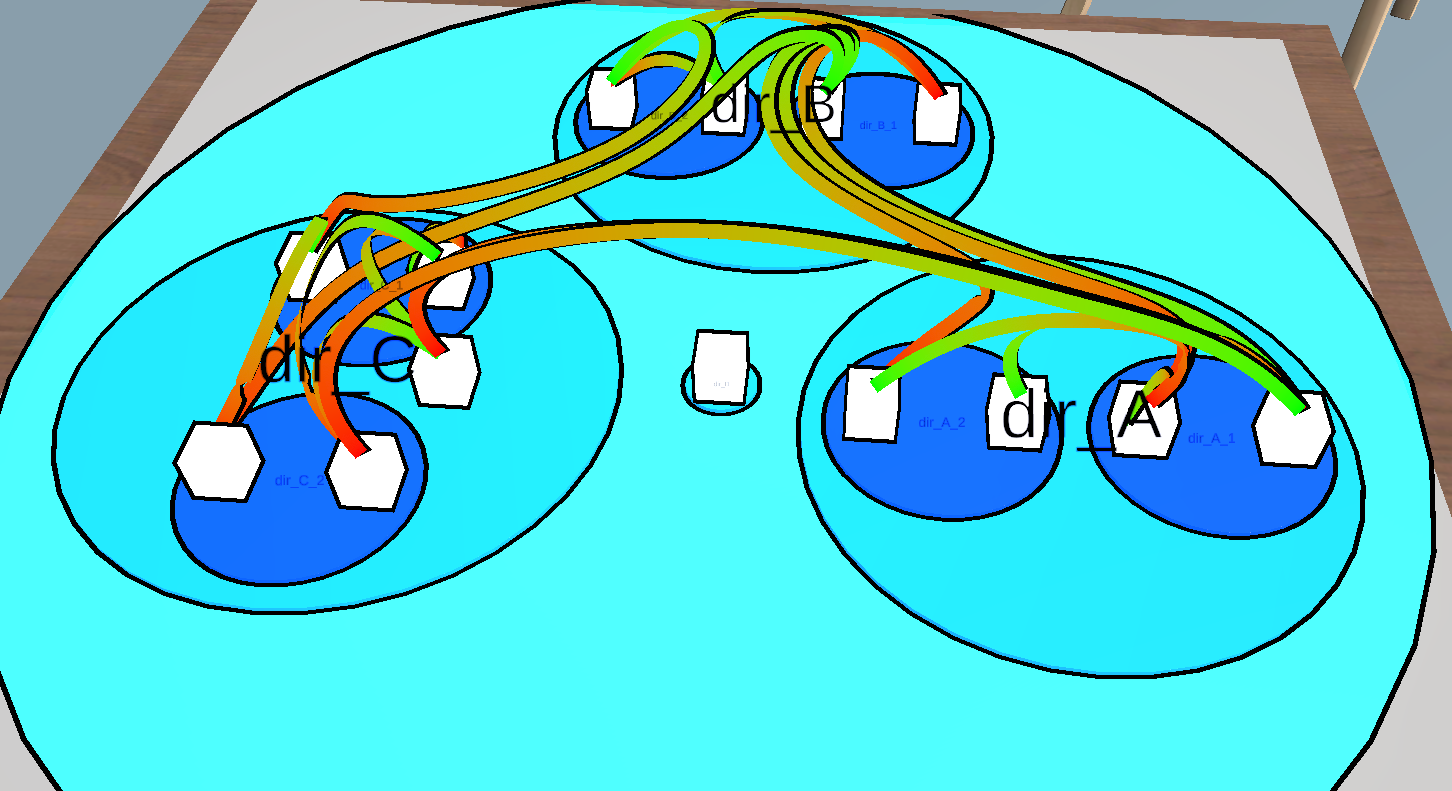
\includegraphics[width=1\textwidth]{Evaluation/img/city_1.png}
  \caption{The first \gls{city} for the user study}\label{fig:city1}
\end{figure}

\begin{figure}[H]
  \centering
  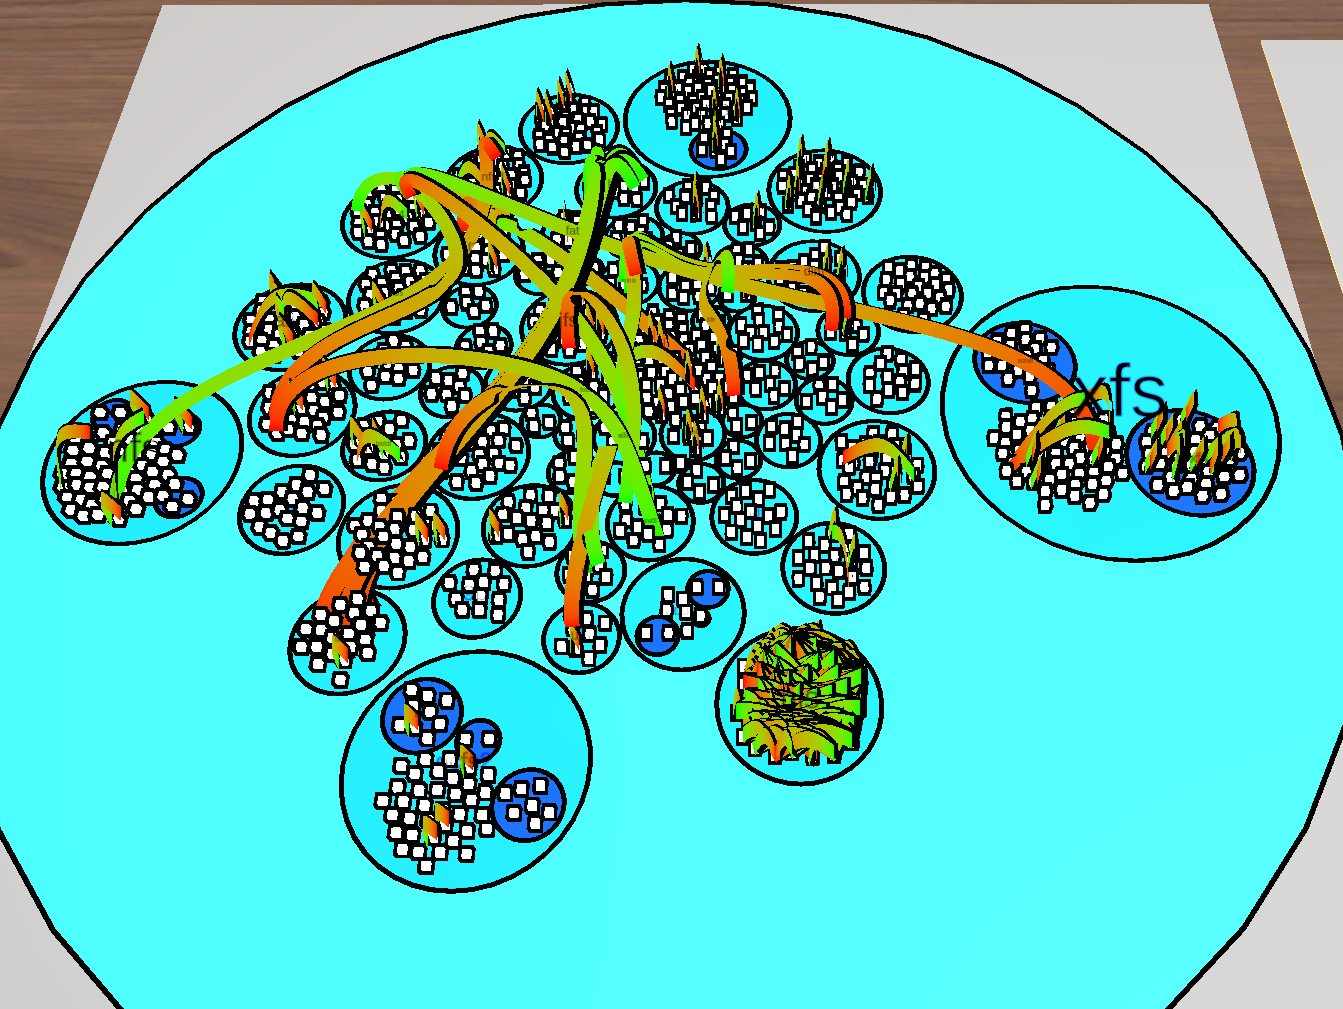
\includegraphics[width=1\textwidth]{Evaluation/img/city_2.png}
  \caption{The second \gls{city} for the user study}\label{fig:city2}
\end{figure}

\begin{figure}[htb]
  \centering
  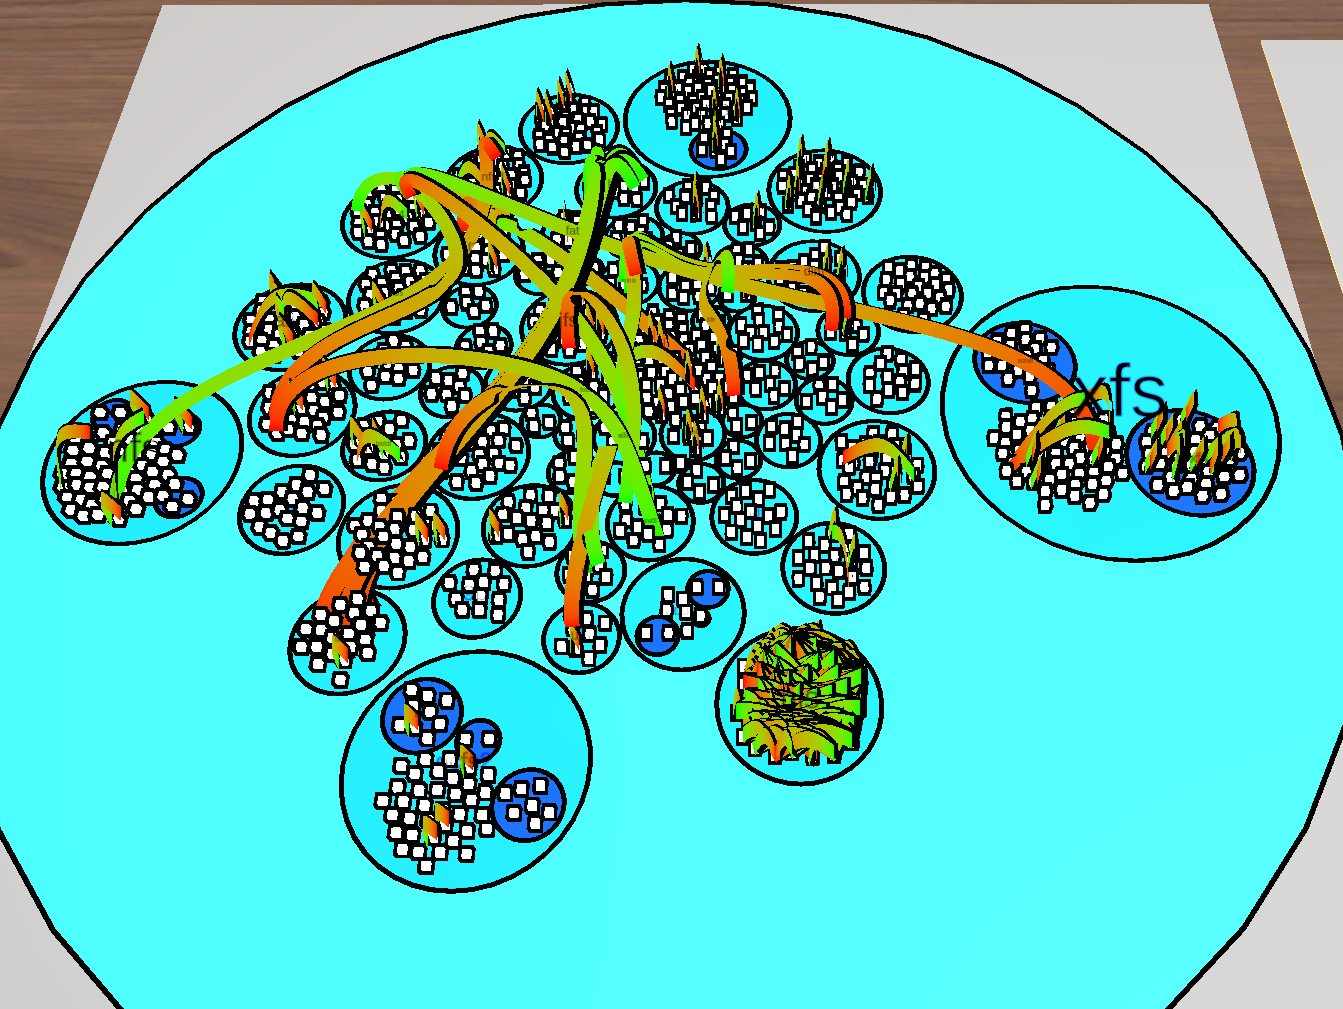
\includegraphics[width=1\textwidth]{Evaluation/img/city_3.png}
  \caption{The third \gls{city} for the user study}\label{fig:city3}
\end{figure}
In this survey the subjects will be asked various demographic questions as well as what Android device and version they will be using.
In addition to that the subjects will be asked if they are experienced with \gls{see} and if they are experienced with software development.
Before the subjects will be asked to solve various tasks they will be asked to watch a short tutorial video on each application.
After the video they will get a training task where every subject can get used to the system and ask questions if they have trouble solving the training task.
The overseer will also make sure that every essential action will be practiced such as zooming and moving the \gls{city}.
Figure \ref{fig:city1} shows a small arranged \gls{city} that shall be used for the training tasks.
The structure of the training \gls{city} is generic and follows a simple pattern.
That shall ensure that the user can focus on the training and that the user does not get overwhelmed.

Following the first questions and the training, the subjects can start with the main tasks.
For each application there will be two tasks and after each task the subjects will be handed a \gls{post-task} questionnaire.
Last but not least there will another questionnaire that aims to scale the \gls{usability} of the two applications.
For the \gls{post-task} questions the \gls{ASQ} will be used and for the \gls{usability} questions \gls{sus} will be used.
Both questionnaires will be discussed later on in section \ref{questionaires}.
For each main task the overseer will also take the completion time of every main task.
The first and second task on the first device will be performed on the \gls{city} that can be seen in figure \ref{fig:city2} and the third and forth task on device two will be performed on the \gls{city} that can be seen on figure \ref{fig:city3}.
These examples are much larger than the training \gls{city} and represent real life code.
The second \gls{city} shows the file system of Linux and the third one shows the network component of Linux.
That way the tasks might reflect better on real world uses for \gls{see}.

To not exhaust the testers too much the experiment shall not take longer than one hour.
This also ensures that there is no to little variance due to exhaustion.
Each participant might have a different concentration span, but this shall not be the focus of this experiment.

\subsection{Realization}
\label{real}
The following sections will cover the realization of the previously planned study. 
The choice of the used survey tool and questionnaires will be explained in section \ref{survey} and section \ref{questionaires}.
Afterwards a pilot study will be executed to test the study and possibly find missing aspects in section \ref{pilot}.
Finally, the final experiment set up will be discussed in section \ref{final}.

\subsubsection{Survey tool}
\label{survey}
As a survey tool Google Forms\footnote{https://www.google.com/forms/about/ (last visit: 05.06.2022)} will be used.
The survey tool has to fulfill the following requirements: 
\begin{itemize}
  \item The study will be online because an overseer has to attend every experiment, and therefore it comes in handy to be flexible in terms of location. For this reason the survey shall be fully in a browser. 
  \item The survey tool should be free to use.
  \item Subjects shall be anonymous.
  \item The results shall be exportable in a data format like \gls{csv}
  \item Subjects should have the option to presave their answers. In addition to that answers should not be lost on reload.
  \item There should be an option to embed the introduction videos in the survey.
\end{itemize}

Google Forms fulfills all these requirements and will therefore be used. 
The final form can be seen in figure \ref{fig:intro} which shows the intro of the survey and in figure \ref{fig:video} which shows the embedded intro video for \gls{see} mobile.
\begin{figure}[H]
  \centering
  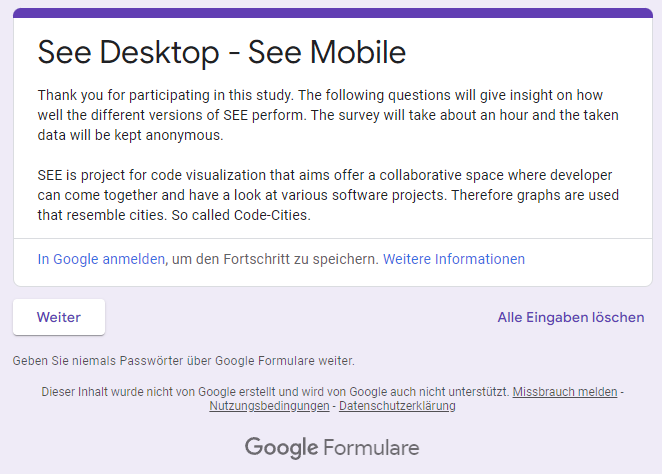
\includegraphics[width=1\textwidth]{Evaluation/img/form_intro.png}
  \caption{The intro of the survey}\label{fig:intro}
\end{figure}

\begin{figure}[H]
  \centering
  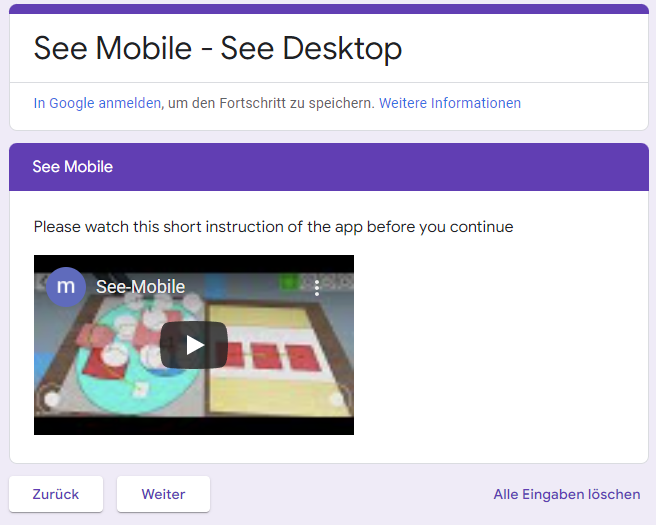
\includegraphics[width=1\textwidth]{Evaluation/img/form_video.png}
  \caption{The introduction video of the survey}\label{fig:video}
\end{figure}

\subsubsection{Questionnaires}
\label{questionaires}
There will be three questionnaires used for the study that will be discussed in detail in the following.
The study will start with a demographic questionnaire that covers general information about the subject.
After every task there will be \gls{ASQ} and after every block of tasks for each of the two covered devices there will be a \gls{sus} questionnaire.
\paragraph{Demographic questionnaire}\mbox{}\\
The subjects shall start the survey with a demographic questionnaire.
\paragraph{Post-task questionnaire}\mbox{}\\
\paragraph{Post-study questionnaire}\mbox{}\\
The \gls{sus} questionnaire was first published in 1986 by John Brooke (\cite{brooke1996sus}) and is therefore widely used and proven as citations in more than 1200 publications up until 2013 show (\cite{brooke2013}).
The \gls{sus} is used in this study for the following advantages: 
\begin{itemize}
  \item It has been made publicly available and is free to use (\cite{brooke1996sus}).
  \item It is widely used and known and therefore already proven to give useful results (\cite{brooke2013}; \cite{lewis2018system}; \cite{grier2013system}).
\end{itemize}
\subsubsection{Pilot study}
\label{pilot}
In a first test the pilot study was executed with one tester.
Afterwards the study was discussed and checked for errors.
It stood out that the example \gls{city} of task one was too different to the one in the second task.
Therefore, the \gls{city} of the first task was exchanged with a larger and better comparable one.
Further on a \gls{city} with 1288 nodes (see figure \ref{fig:city2}) as well as one with 1464 nodes (see figure \ref{fig:city3}) will be used.

Also, the tasks were not comparable because they differed in the types of interactions they used.
In one task the user was asked to rename a node and in the other one the user shall add four nodes.
For renaming a node the user has to use a keyboard which does not make it comparable to just click and add nodes in the second task.

\begin{figure}[htb]
  \centering
  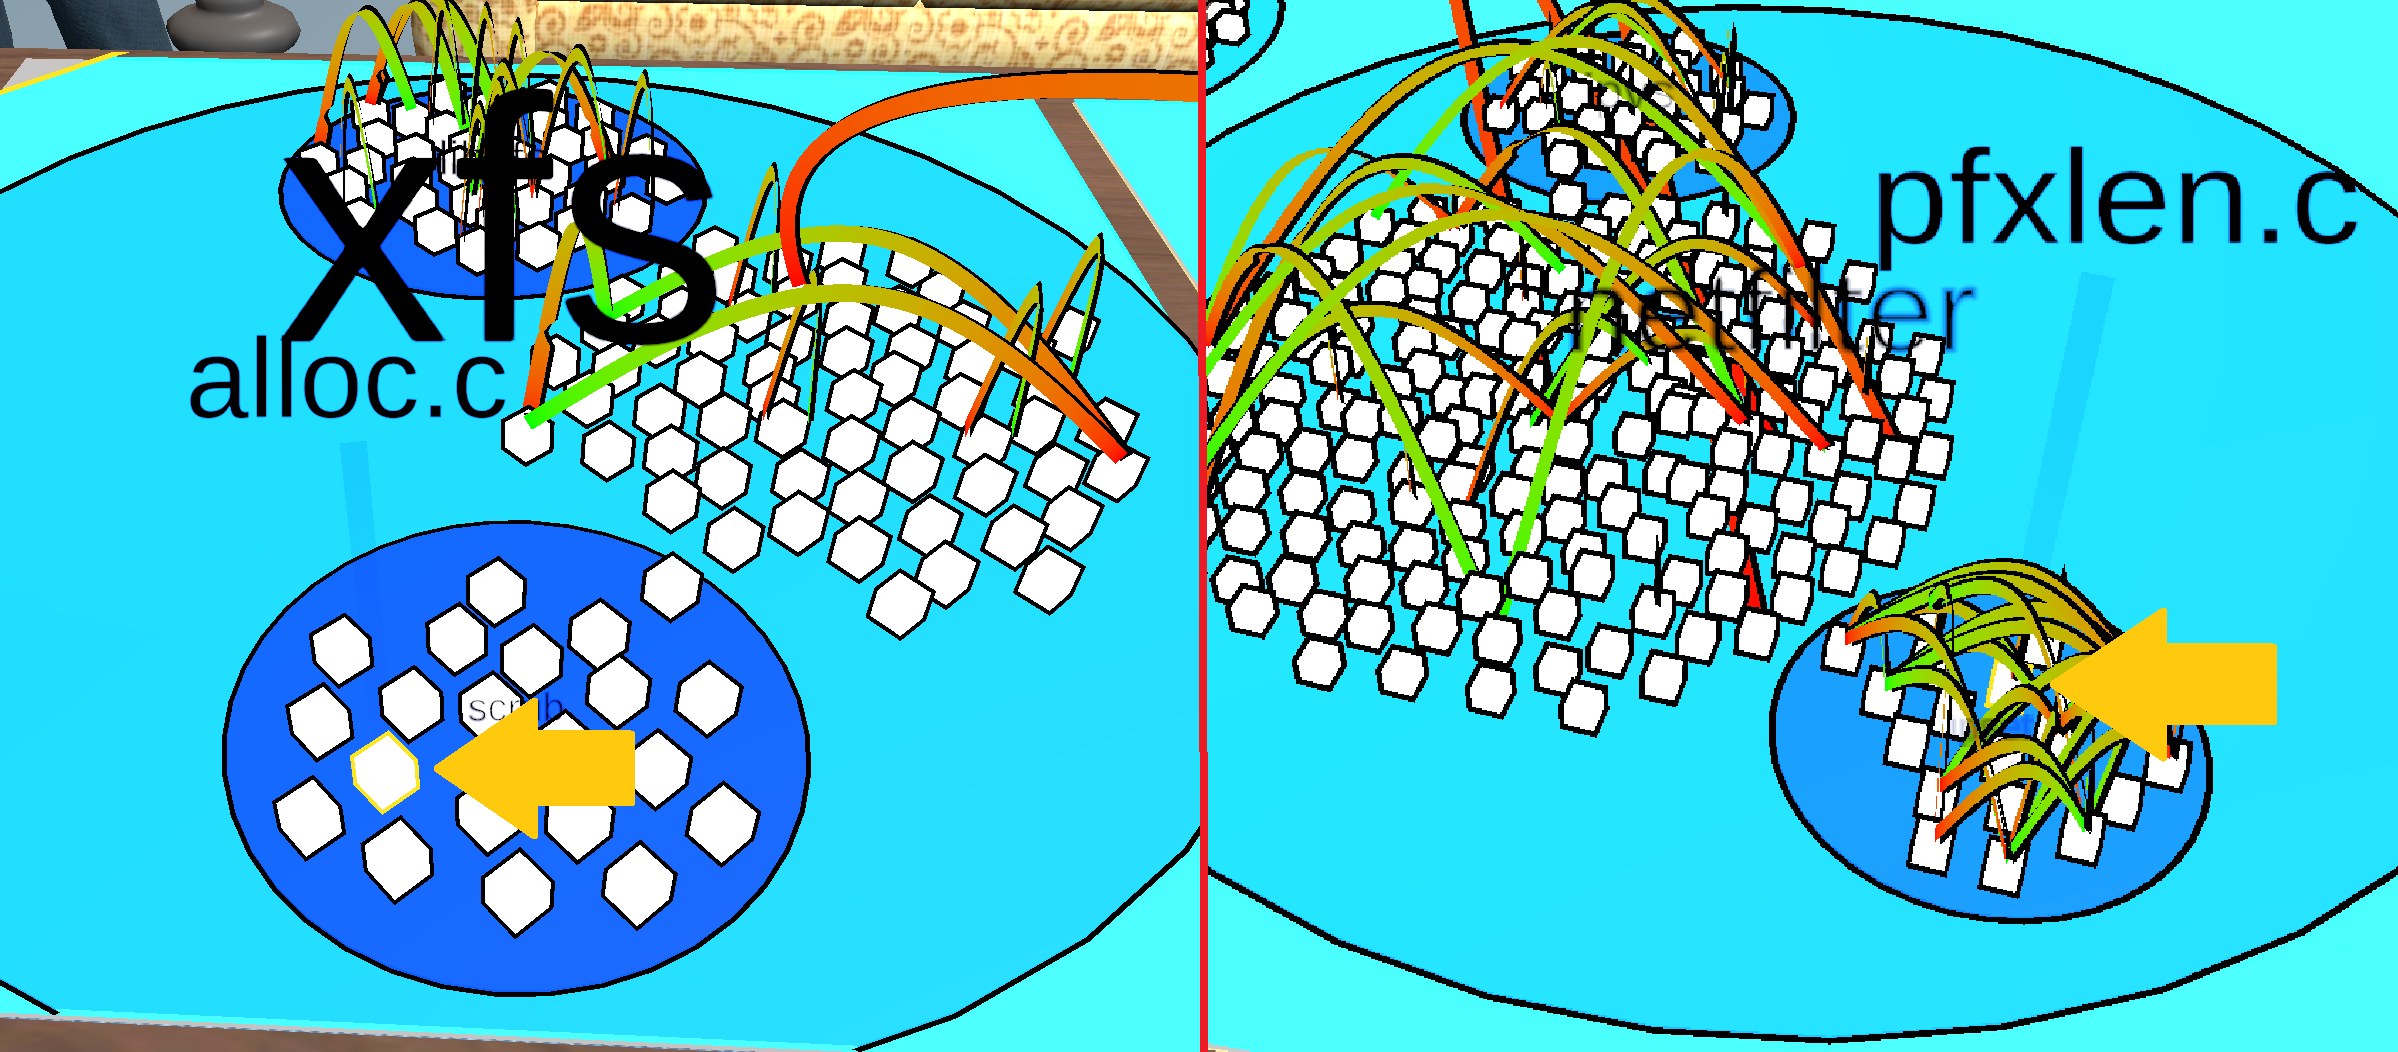
\includegraphics[width=1\textwidth]{Evaluation/img/task1.png}
  \caption{The two key nodes are marked with a yellow arrow}\label{fig:task1}
\end{figure}

\subsubsection{Final experiment set up}
\label{final}
Demographic questions:
\begin{itemize}
  \item Age
        \begin{itemize}
          \item 0-15 years old
          \item 16-30 years old
          \item 31-45 years old
          \item 46+ years old
        \end{itemize}
  \item What gender do you identify as?
        \begin{itemize}
          \item Male
          \item Female
          \item Other ...
          \item Prefer not to say
        \end{itemize}
  \item What is the highest degree or level of education you have completed?
        \begin{itemize}
          \item Some High School (Hauptschule/Realschule...)
          \item High School (Abitur)
          \item Bachelor's Degree
          \item Master's Degree
          \item Ph.D. or higher
          \item Prefer not to say
          \item Other ...
        \end{itemize}
\end{itemize}

Questions regarding used hardware and experience
\begin{itemize}
  \item Are you already experienced with See?
  \item Do or did you play first person video games?
  \item Do or did you develop software?
  \item On which Android device will you attend?
  \item Which Android version are you using?*
\end{itemize}

\begin{table}[]
  \resizebox{\textwidth}{!}{%
    \begin{tabular}{lll}
      Nr.                                                                                                                                                                                         &
      Task                                                                                                                                                                                        &
      Expected time                                                                                                                                                                                 \\ \hline
      Training                                                                                                                                                                                    &
      \begin{tabular}[c]{@{}l@{}}Navigate through the planes "dir\_root" \\ \textgreater "dir\_B" \textgreater "dir\_B\_2". On that plane \\ select "b2\_b.cpp" and rename it "b42".\end{tabular} &
      1 - 5 mins                                                                                                                                                                                    \\
      1                                                                                                                                                                                           &
      \begin{tabular}[c]{@{}l@{}}Detect the largest plane "xfs". On that\\ plane find plane "scrub". Then find \\ and delete node "alloc.c".\end{tabular}                                         &
      0.5 - 5 mins                                                                                                                                                                                  \\
      2                                                                                                                                                                                           &
      \begin{tabular}[c]{@{}l@{}}Find the plane with one blue child \\ plane ("btrfs"). On the blue child \\ plane "tests" add four new nodes.\end{tabular}                                       &
      1 - 5 mins                                                                                                                                                                                    \\ \hline
      Training                                                                                                                                                                                    &
      \begin{tabular}[c]{@{}l@{}}Navigate through the planes "dir\_root" \\ \textgreater "dir\_C" \textgreater "dir\_C\_2". On that plane \\ select "c2\_b.cpp" and rename it "c42".\end{tabular} &
      1 - 5 mins                                                                                                                                                                                    \\
      3                                                                                                                                                                                           &
      \begin{tabular}[c]{@{}l@{}}Detect the \\ largest plane "netfilter". On that plane\\ find plane "ipset". Then find and \\ delete node "pfxlen.c".\end{tabular}                               &
      0.5 - 5 mins                                                                                                                                                                                  \\
      4                                                                                                                                                                                           &
      \begin{tabular}[c]{@{}l@{}}On the plane with the most \\ edges ("ipv6") find the smallest plane\\ "ila" and connect all four nodes on it.\end{tabular}                                      &
      1 - 5 mins                                                                                                                                                                                    \\ \hline
    \end{tabular}%
  }
  \caption{The tasks used for the experiment. The device will be switched after task 2.}
  \label{table:tasks}
\end{table}

\begin{table}[]
  \resizebox{\textwidth}{!}{%
    \begin{tabular}{llll}
      Phase          &                        & \multicolumn{2}{l}{Description}                                          \\ \hline
      Pre-Experiment &                        & \multicolumn{2}{l}{Demographic questionnaire}                            \\ \hline
                     & City                   & Group 1                                       & Group 2                  \\ \hline
      Training       & Figure \ref{fig:city1} & \multirow{6}{*}{Desktop}                      & \multirow{6}{*}{Mobile}  \\
      Task 1         & Figure \ref{fig:city2} &                                               &                          \\
      ASQ            &                        &                                               &                          \\
      Task 2         & Figure \ref{fig:city2} &                                               &                          \\
      ASQ            &                        &                                               &                          \\
      SUS            &                        &                                               &                          \\ \hline
      Training       & Figure \ref{fig:city1} & \multirow{6}{*}{Mobile}                       & \multirow{6}{*}{Desktop} \\
      Task 3         & Figure \ref{fig:city3} &                                               &                          \\
      ASQ            &                        &                                               &                          \\
      Task 4         & Figure \ref{fig:city3} &                                               &                          \\
      ASQ            &                        &                                               &                          \\
      SUS            &                        &                                               &
    \end{tabular}%
  }
  \caption{Experimental procedure per subject. The procedure is swapped per group.}
  \label{table:procedure}
\end{table}


\subsubsection{Execution}